\section{Q3: Convolutional Autoencoders and Representation Probing}
\label{sec:q3}

\subsection{Q3(a): Bottleneck Capacity Sweep and Model Selection}
\paragraph{Symmetrical Convolutional Architecture.}
To investigate unsupervised representation learning, we design a symmetrical convolutional autoencoder where the encoder progressively downsamples the image from $32 \times 32$ to $2 \times 2$ via stride-2 convolutions, followed by a linear projection into bottleneck dimension $d \in \{64, 256, 1024\}$:
\begin{itemize}
    \item \textbf{Encoder:} $\text{Conv}(3 \to 32) \to \text{Conv}(32 \to 48) \to \text{Conv}(48 \to 64) \to \text{Conv}(64 \to 64) \to \text{Flatten} (256\text{-D}) \to \text{Linear}(256 \to d)$.
    \item \textbf{Decoder:} $\text{Linear}(d \to 256) \to \text{Reshape} (64 \times 2 \times 2) \to \text{Deconv}(64 \to 64) \to \text{Deconv}(64 \to 48) \to \text{Deconv}(48 \to 32) \to \text{Deconv}(32 \to 3) \to \text{Sigmoid}$.
\end{itemize}
Outputs are bounded in $[0, 1]$ via Sigmoid to match unit-normalized input images. Training optimizes Mean Squared Error (MSE) loss for $20$ epochs using AdamW ($\eta=10^{-3}$, cosine annealing, batch size $64$, seed $26013$).

\begin{table}[t]
\centering
\caption{Q3(a) Convolutional Autoencoder parameter counts and reconstruction MSE across bottleneck capacities $d \in \{64, 256, 1024\}$. Model selection conducted strictly on the $5{,}000$-sample validation set.}
\label{tab:q3a_mse}
\resizebox{\columnwidth}{!}{
\begin{tabular}{lccccc}
\toprule
\textbf{Bottleneck $d$} & \textbf{Enc Params} & \textbf{Dec Params} & \textbf{Total Params} & \textbf{Val MSE} & \textbf{Test MSE} \\
\midrule
$d = 64$   & $95{,}856$  & $95{,}987$  & $191{,}843$ & $0.008134$ & $0.008159$ \\
$d = 256$  & $145{,}200$ & $145{,}139$ & $290{,}339$ & $0.006373$ & $0.006409$ \\
$\mathbf{d = 1024}$ & $\mathbf{342{,}576}$ & $\mathbf{341{,}747}$ & $\mathbf{684{,}323}$ & $\mathbf{0.005855}$ & $\mathbf{0.005888}$ \\
\midrule
\textbf{DAE ($b=256$)} & $145{,}200$ & $145{,}139$ & $290{,}339$ & $0.007734$ & $0.007760$ \\
\bottomrule
\end{tabular}
}
\end{table}

\begin{figure}[t]
\centering
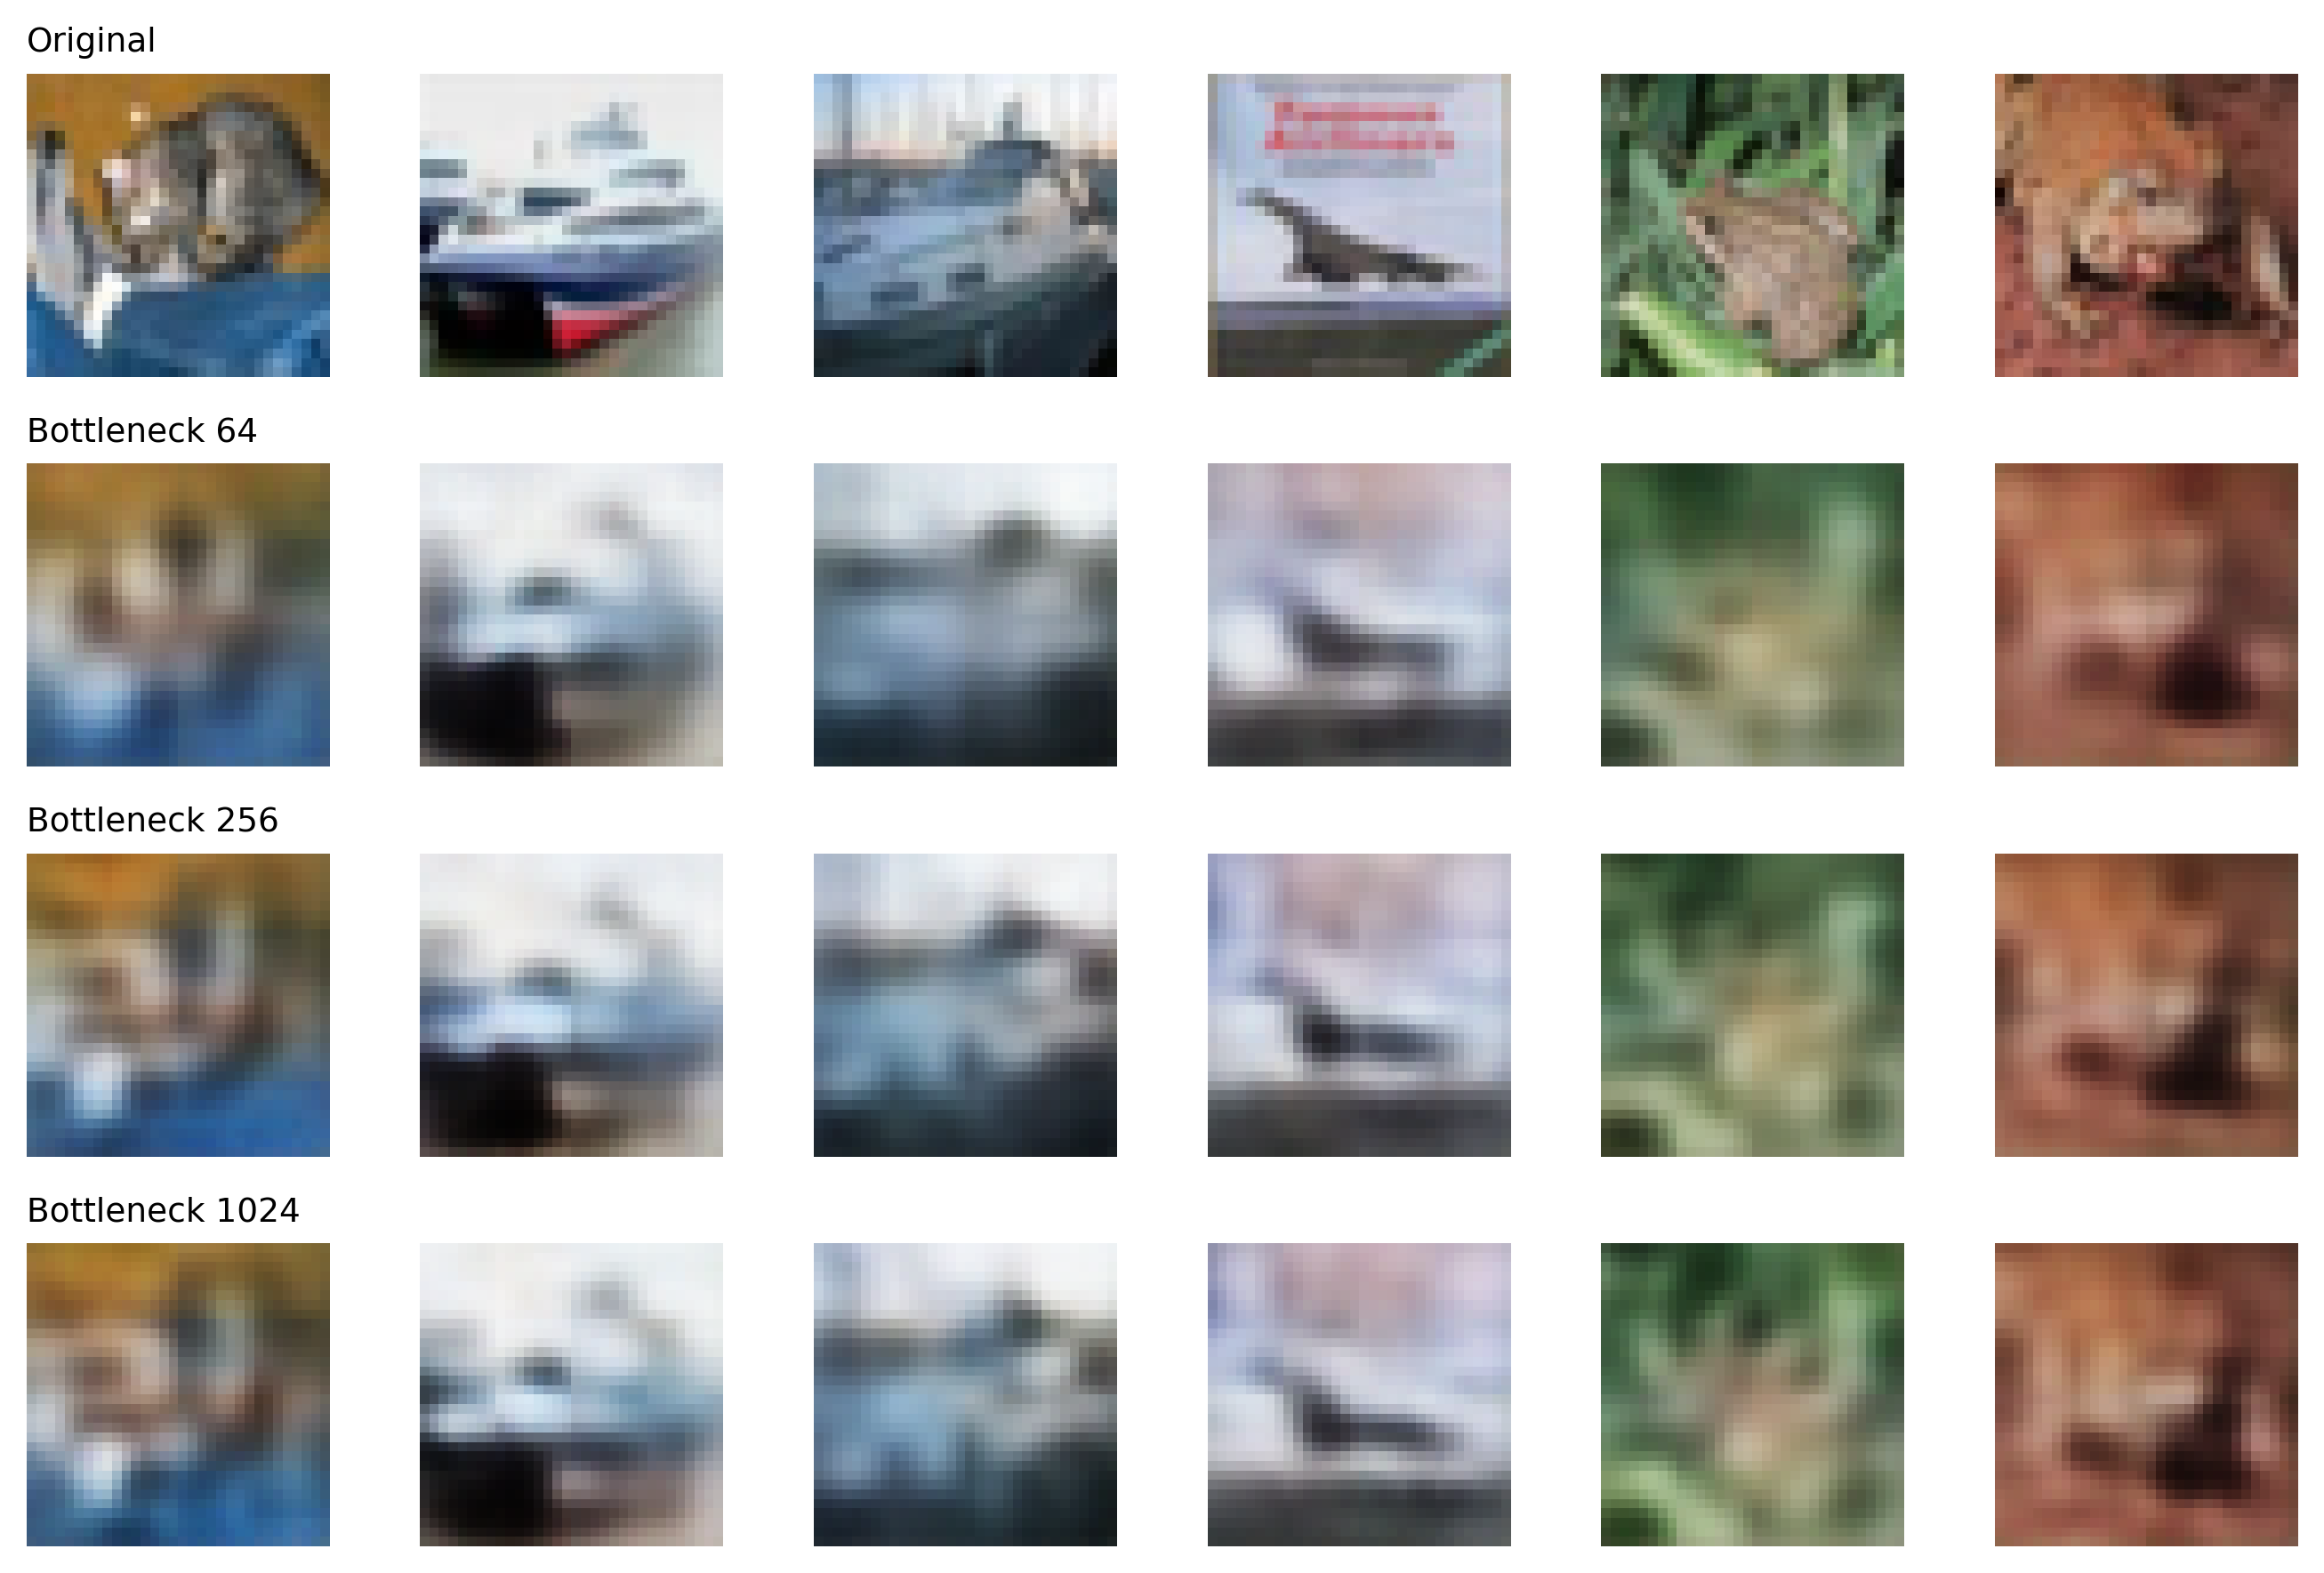
\includegraphics[width=0.78\linewidth]{figures/q3a_reconstruction_grid.png}
\caption{Q3(a) Test image reconstructions across bottleneck capacities $d \in \{64, 256, 1024\}$ compared against original CIFAR-10 inputs.}
\label{fig:q3a_grid}
\end{figure}

\paragraph{Validation-Based Model Selection.}
As required by the experimental integrity protocol, the clean autoencoder was selected strictly using validation reconstruction error (Table~\ref{tab:q3a_mse}):
\begin{equation}
\begin{aligned}
    \text{Val MSE}(1024) &= 0.005855 < 0.006373 \, (b=256) \\
    &< 0.008134 \, (b=64).
\end{aligned}
\end{equation}
Bottleneck $\mathbf{d = 1024}$ was formally selected. The official test set was evaluated strictly post-selection, yielding $\text{Test MSE} = 0.005888$. 

As visualized in Figure~\ref{fig:q3a_grid}, expanding bottleneck capacity allows the network to reconstruct high-frequency texture details and object boundaries that are blurred under $d=64$.

\subsection{Q3(b): Denoising Autoencoder \& Downstream Recovery}
\paragraph{Denoising Protocol.}
We construct a Denoising Autoencoder (DAE) with $b=256$ trained with zero class supervision. The encoder receives corrupted inputs $\tilde{\mathbf{x}} = \text{clip}(\mathbf{x} + \boldsymbol{\epsilon}, 0, 1)$, where $\boldsymbol{\epsilon} \sim \mathcal{N}(\mathbf{0}, \sigma^2 \mathbf{I})$ with $\sigma = 0.2$, while the reconstruction loss is computed strictly against the uncorrupted target image $\mathbf{x}$. The DAE achieves a validation MSE of $0.007734$ and test MSE of $0.007760$.

\begin{figure}[t]
\centering
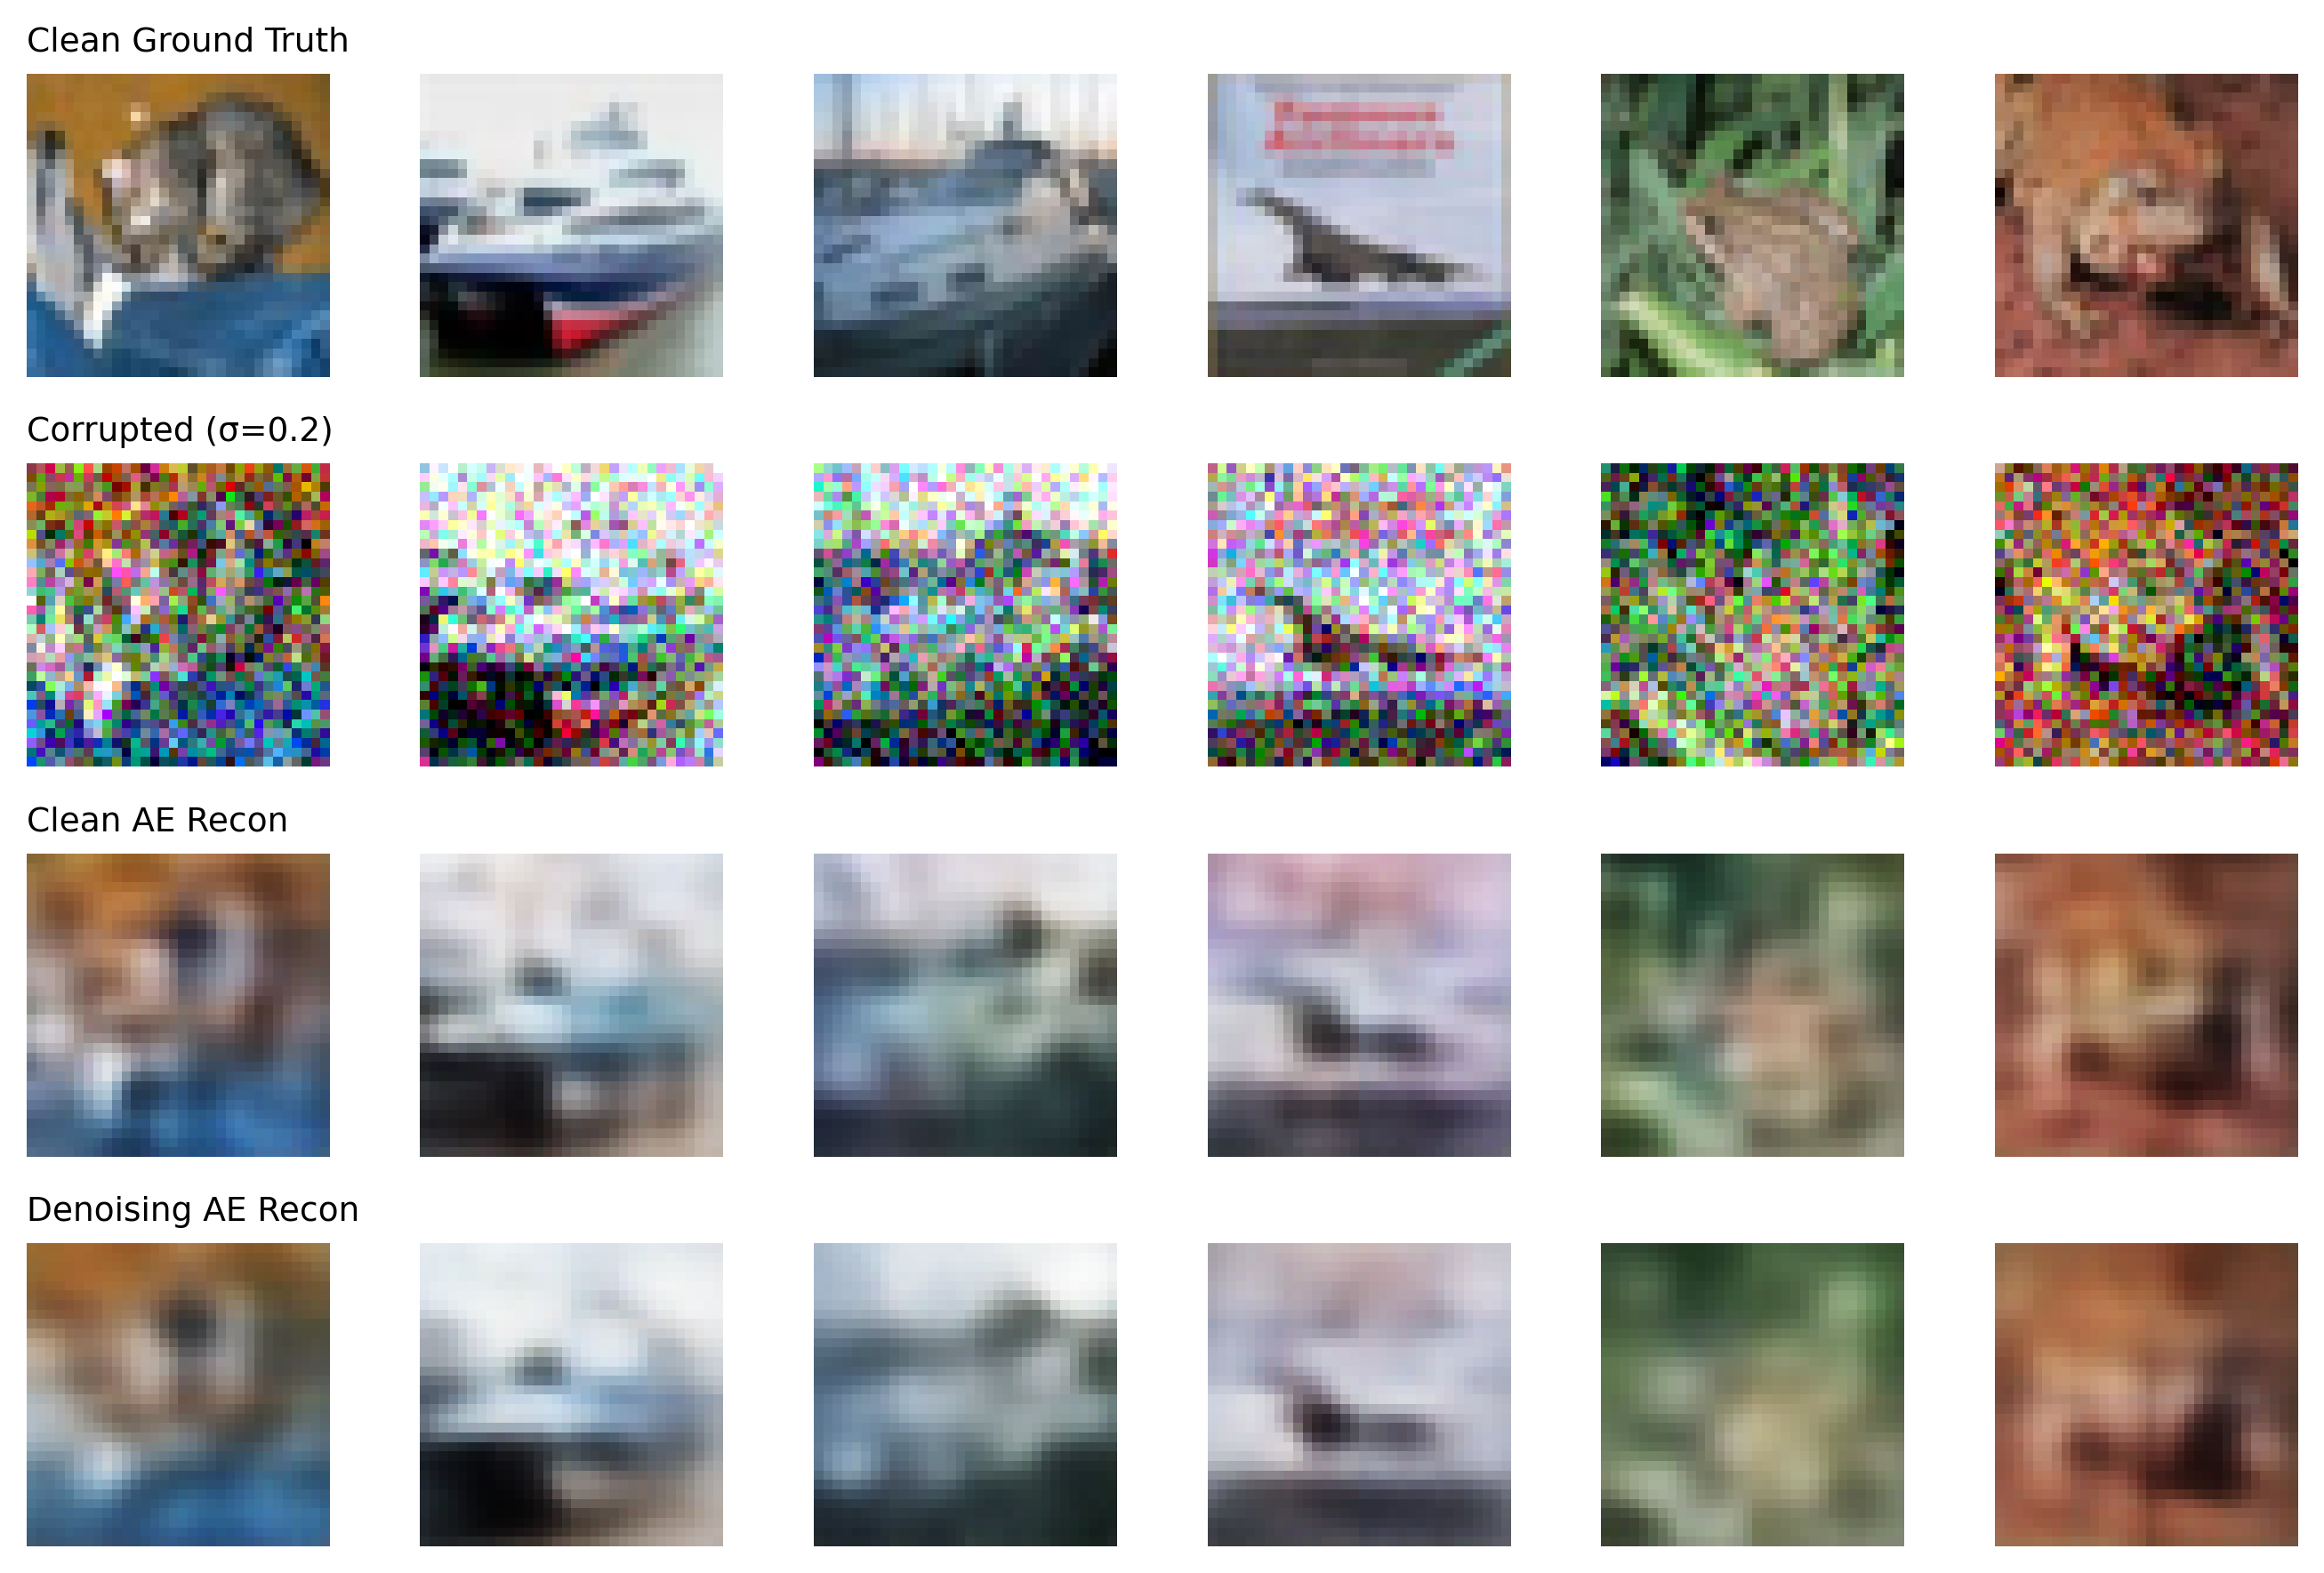
\includegraphics[width=0.78\linewidth]{figures/q3b_denoising_comparison.png}
\caption{Q3(b) Semantic denoising comparison: (Row 1) Clean Ground Truth, (Row 2) Corrupted with $\sigma=0.2$, (Row 3) Clean AE Recon ($b=1024$), (Row 4) DAE Recon ($b=256$).}
\label{fig:q3b_denoise}
\end{figure}

\begin{table}[t]
\centering
\caption{Q3(b) Downstream classification accuracy on the official CIFAR-10 test set using the fixed, frozen FairCNN classifier from Q2(a) ($72.05\%$ clean baseline). Both autoencoders receive identical corrupted test inputs.}
\label{tab:q3b_downstream}
\resizebox{\columnwidth}{!}{
\begin{tabular}{lcc}
\toprule
\textbf{Input Evaluated by Fixed FairCNN} & \textbf{Test Accuracy} & \textbf{Delta vs. Corrupted} \\
\midrule
1. Clean Test Images (Baseline)           & $\mathbf{72.05\%}$ & — \\
2. Corrupted Test Images ($\sigma = 0.2$) Directly & $20.07\%$ & Baseline ($-51.98\%$) \\
3. Clean AE Reconstructions ($b=1024$)    & $27.65\%$ & $\mathbf{+7.58\%}$ \\
4. Denoising AE Reconstructions ($b=256$) & $27.57\%$ & $\mathbf{+7.50\%}$ \\
\bottomrule
\end{tabular}
}
\end{table}

\paragraph{Fixed Downstream Classifier Evaluation.}
To assess whether pixel-level denoising restores semantic utility, we evaluate the reconstructed test images using our fixed, previously trained FairCNN classifier from Q2(a) without retraining or fine-tuning (Table~\ref{tab:q3b_downstream}). 
\begin{enumerate}
    \item \textbf{Susceptibility to Noise:} Directly corrupting images with $\sigma=0.2$ drops CNN classification accuracy from $72.05\%$ to $20.07\%$ (a $-51.98\%$ collapse).
    \item \textbf{Denoising Gain:} Passing corrupted images through either the Clean AE ($27.65\%$) or DAE ($27.57\%$) recovers approximately $+7.5\%$ accuracy over raw corrupted inputs.
    \item \textbf{The Reconstruction Domain Shift:} Despite effective visual smoothing (Figure~\ref{fig:q3b_denoise}), neither autoencoder recovers the clean $72.05\%$ baseline. This exposes a fundamental limitation of unsupervised $L_2$ pixel reconstruction: autoencoders minimize average squared error across all pixels, attenuating sharp edge gradients and high-frequency textures that deep CNN classifiers rely upon for discrimination.
\end{enumerate}

\subsection{Q3(c): Representation Quality vs. Class Information}
\paragraph{Linear Probing Protocol.}
To evaluate the semantic quality of learned representations without fine-tuning, we freeze all encoder weights $\boldsymbol{\theta}_{\text{enc}}^*$ and train a single linear classification layer $\mathbf{y} = \mathbf{W}\mathbf{z} + \mathbf{b}$ on the extracted bottleneck features. Feature standardization $(\boldsymbol{\mu}, \boldsymbol{\sigma})$ is fitted exclusively on training representations. Optimal learning rates and early stopping are determined strictly on validation representations before single test evaluation.

\begin{figure}[t]
\centering
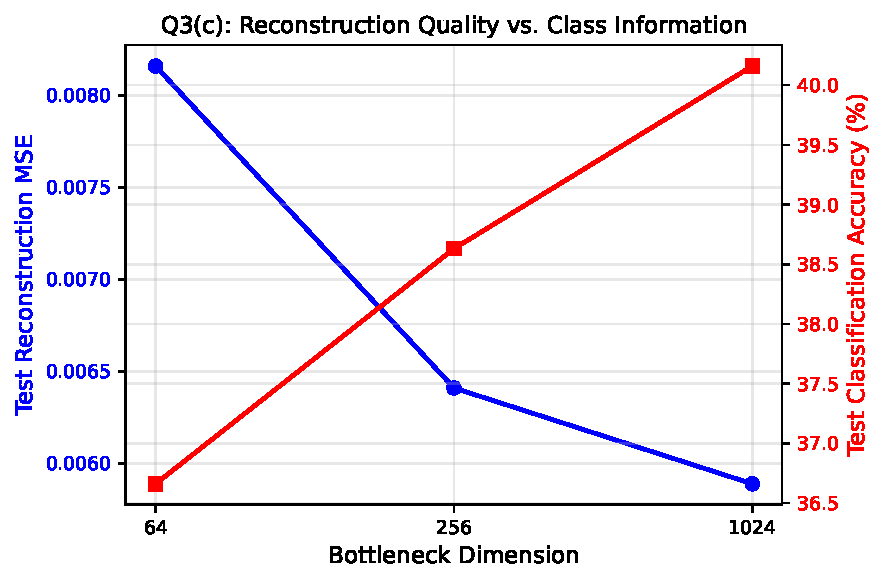
\includegraphics[width=0.78\linewidth]{figures/q3c_reconstruction_vs_class_info.pdf}
\caption{Q3(c) Dual-axis trade-off curve: Test Reconstruction MSE (blue, lower is better) vs. Frozen Linear Probe Test Accuracy (red, higher is better) across bottleneck capacities $d \in \{64, 256, 1024\}$.}
\label{fig:q3c_tradeoff}
\end{figure}

\begin{table}[t]
\centering
\caption{Q3(c) Frozen linear probe classification accuracy and test reconstruction MSE across autoencoder bottlenecks.}
\label{tab:q3c_probe}
\resizebox{\columnwidth}{!}{
\begin{tabular}{lcccc}
\toprule
\textbf{Feature Backbone} & \textbf{Bottleneck $d$} & \textbf{Test MSE} & \textbf{Probe Val Acc} & \textbf{Probe Test Acc} \\
\midrule
Clean AE  & $64$   & $0.008159$ & $36.28\%$ & $36.66\%$ \\
Clean AE  & $256$  & $0.006409$ & $39.32\%$ & $38.63\%$ \\
Clean AE  & $1024$ & $\mathbf{0.005888}$ & $\mathbf{40.16\%}$ & $\mathbf{40.16\%}$ \\
\midrule
DAE       & $256$  & $0.007760$ & $39.30\%$ & $38.77\%$ \\
\bottomrule
\end{tabular}
}
\end{table}

\paragraph{Analysis of Reconstruction vs. Class Information.}
As illustrated in Figure~\ref{fig:q3c_tradeoff} and Table~\ref{tab:q3c_probe}:
\begin{itemize}
    \item \textbf{Monotonic Correlation:} Across clean autoencoders, reconstruction MSE and linear probe accuracy are monotonically aligned: as $d$ expands from $64 \to 1024$, reconstruction error drops from $0.00816 \to 0.00589$, while linear probe test accuracy increases from $36.66\% \to 40.16\%$. A wider bottleneck retains more linearly separable class variance.
    \item \textbf{DAE Compactness:} Notably, the DAE ($b=256$) achieves $38.77\%$ probe accuracy—slightly outperforming the clean AE of identical dimension ($38.63\%$) despite exhibiting higher reconstruction MSE ($0.00776$ vs. $0.00641$). Denoising forces the encoder to discard independent pixel noise, yielding a more robust semantic subspace.
    \item \textbf{The Linear Separability Gap:} Even at $d=1024$, linear probe accuracy reaches only $40.16\%$, far below end-to-end FairCNN ($72.05\%$). Unsupervised reconstruction allocates representational capacity equally to background pixels and foreground objects, proving that pixel-level reconstruction fidelity is insufficient for high-level semantic categorization.
\end{itemize}
